\documentclass[12pt, letterpaper, twocolumn]{article}
\usepackage[utf8]{inputenc}
\usepackage{graphicx} %display images
\usepackage{hyperref} %clickable links
\usepackage{listings}
\usepackage{color}
 
\title{Procesamiento de Grafos}
\author{Daniela Vignau León}
\date{30 de octubre de 2019}

\definecolor{airforceblue}{rgb}{0.36,0.54,0.66}
\definecolor{gray}{rgb}{0.5,0.5,0.5}
\definecolor{ceruleanblue}{rgb}{0.16,0.32,0.75}

\lstset{frame=tb,
  language=Java,
  aboveskip=3mm,
  belowskip=3mm,
  showstringspaces=false,
  columns=flexible,
  breaklines=true,
  basicstyle={\small\ttfamily},
  numbers=none,
  numberstyle=\tiny\color{gray},
  keywordstyle=\color{blue},
  commentstyle=\color{airforceblue},
  stringstyle=\color{ceruleanblue},
  breaklines=true,
  breakatwhitespace=true,
  tabsize=3
}
 
\begin{document}

\maketitle
 
\begin{abstract}
En el presente trabajo, se pretende mostrar al lector cómo realizar el procesamiento de grafos obtenido a partir de un \textit{dataset} de la librería de SNAP.
\end{abstract}

\begin{description}
\item [{1.Introduction}]~
\end{description}

De manera general, un grafo está definido como \textit{G = (V, E)} donde V representa a los vértices y E a las aristas. Existen muchos tipos:
\begin{itemize}
	\item Dirigidos
	\item No dirigidos
	\item Con peso
	\item ... y muchos otros más.
\end{itemize}

Los grafos tienen aplicaciones en muchísimas áreas que permiten resolver diversos problemas; como modelar trayectos, administración de proyectos, encontrar los caminos más cortos u óptimos e inclusive para el estudio de las redes sociales. 

A esto último se le conoce como \textit{Análisis de redes sociales} donde se mapean las relaciones entre personas, grupos, organizaciones, URLs y otros tipos de información. Los vértices representan a las personas y los grupos, y las aristas muestran la relación entre los nodos. 

Para el presente trabajo, se utilizó la libería de SNAP (Standford Network Analysis Platform) la cual permite la fácil manipulación y análisis de redes grandes en lenguajes de programación como C++ y Python. Es importante notar que ésta debe de estar previamente \href{https://snap.stanford.edu/snap/install.html}{descargada} e instalada. Asimismo se descargó un \textit{dataset} proporcionado por SNAP el cual se puede descargar \href{https://snap.stanford.edu/data/index.html}{aquí}.

\begin{description}
\item [{2. Importación del grafo}]~
\end{description}

Después de haber seleccionado el dataset con el que se quiere trabajar, se debe de descargar y extraer el archivo que tiene la extensión \textit{.txt.gz} a la carpeta que contendrá el proyecto. En este caso se seleccionó la base de datos de \textbf{wiki-Vote}, si se desea descargar otro dataset, se tendrán que hacer unas modificaciones mínimas.

Dentro del proyecto, se deberá crear un gráfo para poder llamarlo en los diferentes métodos. Dentro del main, se deberá insertar la siguiente línea: 
\begin{lstlisting}
Dgraph graph = TSnap::LoadEdgeList<DGraph> ("wiki-Vote.txt", 0, 1)
\end{lstlisting}

\begin{description}
\item[{3. Creación de métodos}]~
\end{description}

El usuario deberá de crear los métodos para la exportación del grafo en los diferentes formatos que se requieran. De manera general, se deberá de abrir un archivo con la extensión requerida para escribir el grafo exportado. Se debe de tener mucho cuidado en cómo leen los formatos los grafos, pues es ahí donde radica la manera en la que se ve o no el grafo. 

\begin{description}
\item[{4. Resultados}]~
\end{description}

Con el simple propósito de comparar uno u otro formato, se calculó el tiempo de ejecución en milisegundos de cada uno de los métodos. Los resultados fueron: 

\begin{table}[ht]
\center
\begin{tabular}{ |c| c| }
\hline
	\textbf{Formato} & \textbf{Tiempo de Ejecución} \\ 
\hline
	GraphML & 108.674 ms \\  
\hline
	GEXF & 116.105 ms \\
\hline
	GDF & 96.175 ms \\
\hline
	JSON & 104.142 \\
\hline
\end{tabular}

\caption{Tabla de tiempos de ejecución}
\label{table:1}
\end{table}

En este caso se decidió graficar el formato GraphML para poder visualizar la gráfica en un software llamado \textit{Gephi}. Se debe de descargar el software, inicializarlo y seleccionar qué archivo se quiere abrir. Una vez realizado esto, el grafo será creado y se verá de la siguiente manera:

\begin{figure}[ht]
\center
	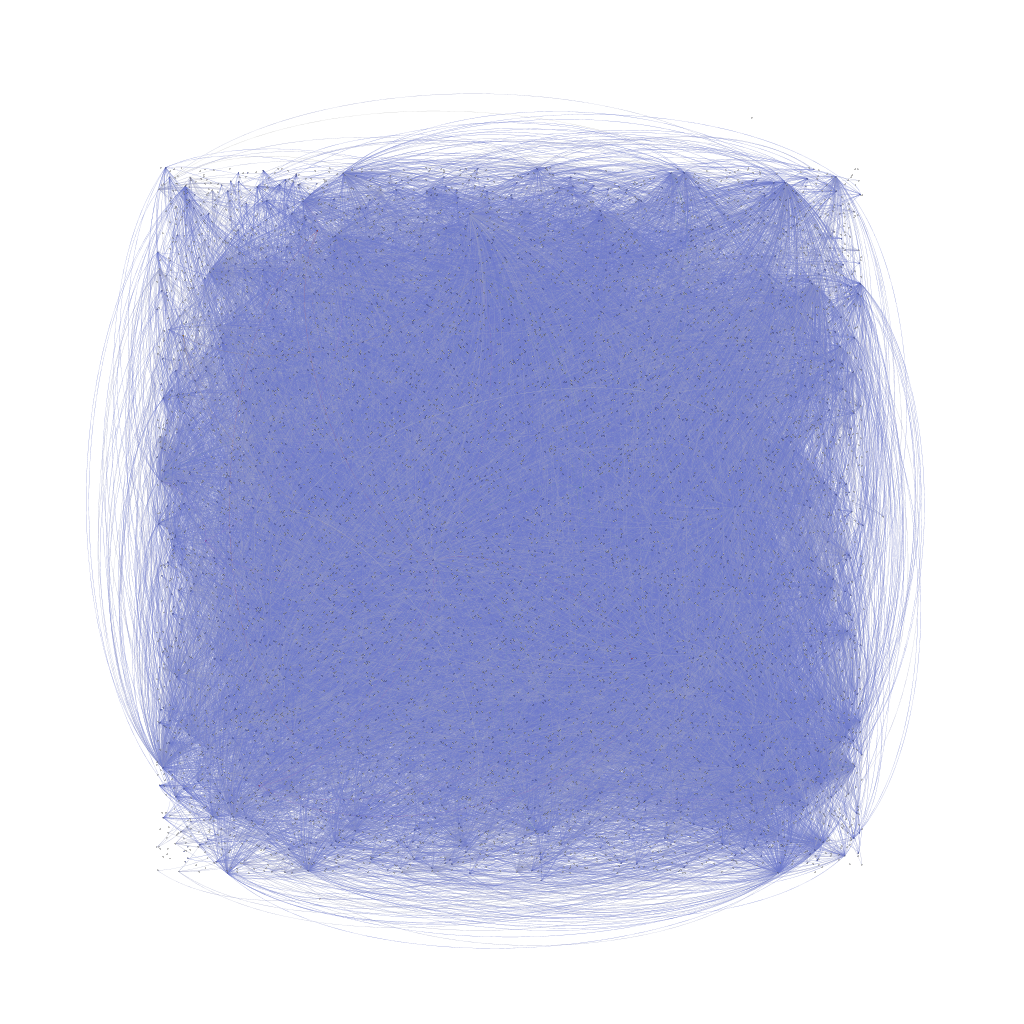
\includegraphics[width = 4cm, height = 4cm]{finalgraph} % Image of the graph	
	\caption{Grafo del dataset de wiki-Vote}
	\label{fig:graph}

\break
	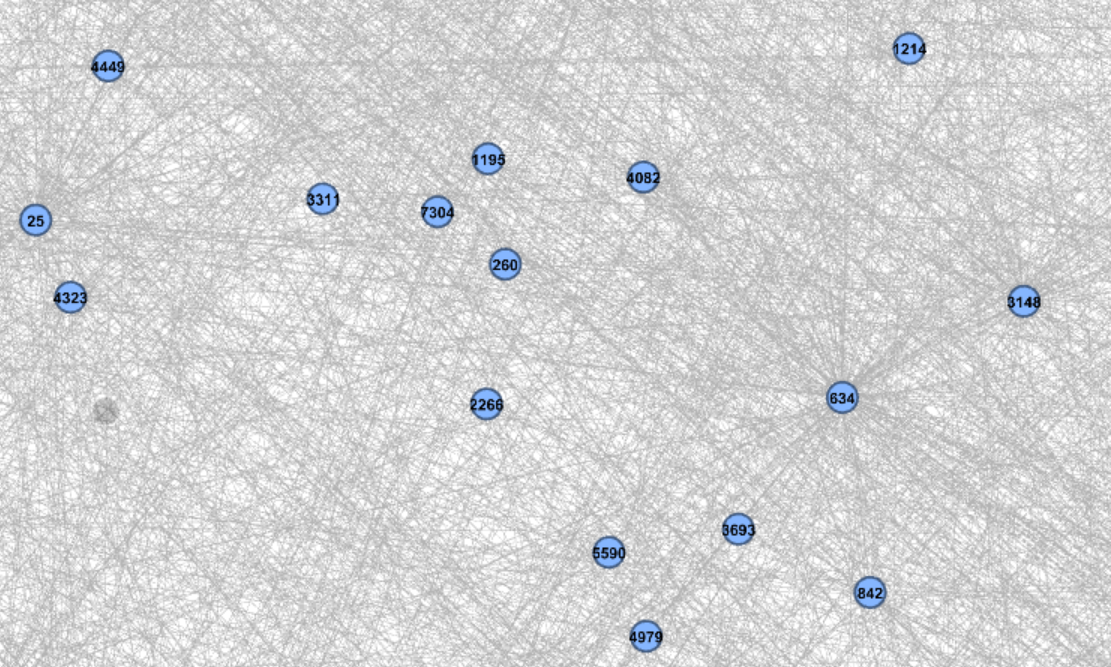
\includegraphics[width = 6cm, height = 4cm]{closeup} % Image of the graph	
	\caption{Acercamiento del mismo grafo}
\end{figure}


\begin{description}
\item[{5. Interpretación de resutlados}]~
\end{description}

Con respecto a los tiempos de ejecución, se puede apreciar que \textit{GEXF} fue el formato más lento para exportar el grafo, y el más rápido fue \textit{GDF}. 

Se pueden obtener datos interesantes con respecto al grafo utilizando el software anteriormente mencionado. Algunos de ellos son: el camino promedio entre los nodos es de 3.341, el coeficiente promedio de agrupamiento de nodos es de 0.081, la densidad del grafo es de 0.002 y el grafo tiene una modularidad de 0.43. En la figura 2, se muestra un acercamiento del grafo para que el lector pueda, de cierta manera, apreciar cómo es que se ven los vértices conectados así como las etiquetas de cada uno de los nodos. 

\begin{description}
\item[{6. Ventajas y desventajas}]~
\end{description}

\textbf{\emph{Sobre los formatos}}

\textbf{GraphML:} \textit{Ventajas:} Permite añadir atributos a vértices y aristas, grafos jerárquicos. \textit{Desventajas:}  No soporta sub-grafos ni \textit{hiper bordes.}

\textbf{GEXF:} \textit{Ventajas:} Permite especificar atributos dados por el usuario (como peso de los nodos y direcciones de las aristas). \textit{Desventajas:}  Es un archivo pesado.

\textbf{GDF:} \textit{Ventajas:} Permite añadir atributos a vértices y aristas, el documento está dividido entre esos dos. Fácil de leer y de convertir a CSV. \textit{Desventajas:}  Puede llegar a ser un poco pesado,

\textbf{JSON:} \textit{Ventajas:}:El esquema es muy flexible, fácil de leer y dado que es map-based facilita el envío de datos en aplicaciones Web, por ejemplo. \textit{Desventajas:} No es muy práctico utilizarlo para aplicaciones Web ya que puede duplicar información. 

La complejidad temporal de los cuatro formatos es de O(V + E), donde V se refiere a los vértices (nodos) y E a las aristas y todos cuentan con una complejidad espacial de S(1).
\break

\textbf{\emph{Sobre la visualización de grafos}}

Quizás una de las ventajas más grandes de poder visualizar un cierto grafo, en Gephi por ejemplo, es poder darse una idea sobre la distribución de los datos e inclusive se podría llegar a ciertas conclusiones con esto. Otra de las grandes ventajas, es que es realmente fácil encontrar datos como los que se mencionaron en la sección 5: camino promedio entre nodos, coeficiente de agrupamiento, etc. 

Una gran desventaja es que es difícil manipular cientos de miles de datos y que a menos que el usuario tenga una buena idea sobre qué quiere saber del grafo, podrá hacer uso de todas las herramientas. Puede llegar a suceder que se deben de descargar más softwares para visualizar el grafo, porqe al menos Gephi, no permite el formato JSON.


\begin{description}
\item[{7. Código}]~
\end{description}

\begin{lstlisting}
// Exportando a GraphML 
void GraphML(DGraph graph) {
  ofstream file ("wiki_vote.graphml");
  if (file.is_open()) {
      file << "<?xml version=\"1.0\" encoding=\"UTF-8\"?>\n";
      file << "<graphml xmlns=\"http://graphml.
      graphdrawing.org/xmlns\" xmlns:xsi=
      \"http://www.w3.org/2001/
      XMLSchema-instance\"xsi:schemaLocation
      =\"http://graphml.graphdrawing.org/
      xmlnshttp://graphml.graphdrawing.org
      /xmlns/1.0/graphml.xsd\">\n";
      file << "<graph id=\"G\" edgedefault=\"directed\">\n";

      for (DGraph::TObj::TNodeI NI = graph->BegNI(); NI < graph->EndNI(); NI++)
			file << "<node id=\"" << NI.GetId() << "\"/>\n";

      int i = 1;
      for (DGraph::TObj::TEdgeI EI = graph->BegEI(); EI < graph->EndEI(); EI++, ++i)
      file << "<edge id=\"e" << i << "\" source=\"" << EI.GetSrcNId() << "\" target=\"" << EI.GetDstNId() << "\"/>\n";
      file << "</graph>\n";
      file << "</graphml>\n";
      file.close();
  }
}

//Exportando a GEXF
void GEXF(DGraph graph) {
	ofstream file ("wiki_vote.gexf");
	if (file.is_open()) {
		file << "<?xml version=\"1.0\" encoding=\"UTF-8\"?>\n";
		file << "<gexf xmlns=\"http://www.gexf.net/1.2draft\" version=\"1.2\">\n";
		file << "<graph mode=\"static\" defaultedgetype=\"directed\">\n";

		file << "<nodes>\n";
		for (DGraph::TObj::TNodeI NI = graph->BegNI(); NI < graph->EndNI(); NI++)
			file << "<node id=\"" << NI.GetId() << "\" />\n";
		file << "</nodes>\n";

		file << "<edges>\n";
		int i = 1;
		for (DGraph::TObj::TEdgeI EI = graph->BegEI(); EI < graph->EndEI(); EI++, ++i)
			file << "<edge id=\"" << i << "\" source=\"" << EI.GetSrcNId() << "\" target=\"" << EI.GetDstNId() << "\" />\n";
		file << "</edges>\n";

		file << "</graph>\n";
		file << "</gexf>\n";
		file.close();
	}
}

//Exportando a GDF
void GDF(DGraph graph) {
	ofstream file ("wiki_vote.gdf");
	if (file.is_open()) {
		file << "nodedef>id VARCHAR\n";
		for (DGraph::TObj::TNodeI NI = graph->BegNI(); NI < graph->EndNI(); NI++)
			file << NI.GetId() << "\n";

		file << "edgedef>source VARCHAR, destination VARCHAR\n";
		for (DGraph::TObj::TEdgeI EI = graph->BegEI(); EI < graph->EndEI(); EI++)
			file << EI.GetSrcNId() << ", " << EI.GetDstNId() << "\n";

		file.close();
	}
}

//Exportando a JSON
void JSON(DGraph graph) {
  ofstream file ("wiki_vote.json");
	if (file.is_open()) {
		file << "{ \"graph\": {\n";
		file << "\"nodes\": [\n";
		for (DGraph::TObj::TNodeI NI = graph->BegNI(); NI < graph->EndNI();) {
			file << "{ \"id\": \"" << NI.GetId() << "\" }";
			if (NI++ == graph->EndNI())
				file << " ],\n";
			else
				file << ",\n";
		}

		file << "\"edges\": [\n";
		for (DGraph::TObj::TEdgeI EI = graph->BegEI(); EI < graph->EndEI();) {
			file << "{ \"source\": \"" << EI.GetSrcNId() << "\", \"target\": \"" << EI.GetDstNId() << "\" }";
			if (EI++ == g->EndEI())
				file << " ]\n";
			else
				file << ",\n";
		}
		file << "} }";
		file.close();
	}
}
\end{lstlisting}

El código para realizar este proyecto puede ser encontrado dando click \href{https://github.com/tec-csf/tc2017-t4-otono-2019-dvigleo}{aquí}.

\begin{thebibliography}{7}
\bibitem{key-2}\textit{\textcolor{black}{\footnotesize{}Jbmusso. 2016. GraphSON Reader and Writer Library. Github. Retrieved October 25, 2019 from https://github.com/tinkerpop/blueprints/wiki/GraphSON-Reader-and-Writer-Library}}{\footnotesize \par}

\bibitem{key-3}\textit{\textcolor{black}{\footnotesize{}Gephi. GraphML Format. Retrieved October 25, 2019 from https://gephi.org/users/supported-graph-formats/gdf-format/}}{\footnotesize \par}

\bibitem{key-4}\textit{\textcolor{black}{\footnotesize{}FileInfo. GEFX file Extension. Retrieved October 25, 2019 from https://fileinfo.com/extension/gexf .}}{\footnotesize \par}

\bibitem{key-5}\textit{\textcolor{black}{\footnotesize{}FALCOR. JSON Graph. Retrieved October 25, 2019 from https://netflix.github.io/falcor/documentation/jsongraph.html}}{\footnotesize \par}

\bibitem{key-6}\textit{\textcolor{black}{\footnotesize{}Gephi. GDF Format. Retrieved October 25, 2019 from https://gephi.org/users/supported-graph-formats/gdf-format/}}{\footnotesize \par}

\bibitem{key-7}\textit{\textcolor{black}{\footnotesize{}Tim Sheard. 2009. Graphs in Computer Science. Retrieved October 25, 2019 from http://web.cecs.pdx.edu/~sheard/course/Cs163/Doc/Graphs.html/ }}{\footnotesize \par}

\bibitem{key-8}\textit{\textcolor{black}{\footnotesize{}Orgnet. Social Network Analysis: An Introduction. Retrieved October 25, 2019 from http://www.orgnet.com/sna.html}}{\footnotesize \par}
\end{thebibliography}

\end{document}